
\chapter{Testování a evaluace}

V této kapitole je popsáno jak je celá aplikace otestována. Dále pak porovnání odhadů zpoždění se stávajícím řešení.

\section{Testování softwarového řešení}

Kód práce popsaný v kapitole \ref{chapter:implementace} je otestován unit testy. Propojení  tohoto softwaru s databází i zdrojem vstpuních dat je testováno integračními testy.

\subsection{Unit testy}

Unit testy testují spravnou funkčnost jednotlivých metod všech softwarových komponent této práce.

Pro ověření správné funkčnosti některých metod jsou vygenerována vstupní či výstupní data. To z důvodu, že tyto metody pracují z komplexní datovou strukturou nebo s velkým objemem dat, který není možno zadat jako vstupní přímo v kódu testu, resp. je potřeba porovnat výstup tetované metody a ze stejných důvodů není možné uvádět výstupní hodnoty pro porovnání přímo v kódu testu. Typickým příkladem takové vstupní struktury je model profilu jízdy, ptotože je potřeba otestovat funkce, které s takovým modelem pracují.

\subsection{Integrační testy}

TODO Popisovat co testují testy? Není v tom žádná složitá logika. Dále otázka k celému textu jak odkazovat na jednotlivé soubory s kodem?

\subsection{Testy kvality}

Všechny následující výkonostní testy jsou prováděny na osobním notebooku s technickými parametry uvedenými v tabulce \ref{table:hw}', kde všechny procesy aplikace včetně databáze běží paralelně.

\begin{center}
	\begin{table}[ht]
\centering
\begin{tabular}{|c|c|}
\hline
 Parametr & Hodnota \\ \hline \hline
 Procesor & 4x Intel(R) Core(TM) i7 CPU @ 2.70 GHz\\ \hline
 Paměť & 16 GB DDR3 RAM  \\  \hline
 Rychlost zápisu na disk & 1000--3000 MB/Sec \\ \hline
 OS & macOS Big Sur\\ \hline
 MySQL & version 8.0.18\\ \hline
\end{tabular}
\label{table:hw}
\end{table}
\end{center}
\footnote{https://9to5mac.com/2016/11/01/the-late-2016-entry-level-13-macbook-pro-has-a-ridiculously-fast-ssd/}
\bigbreak

Pro potlačení zkreslení testů vlivem čekání na stažení dat z internetu jsou všechny data načítána z disku počítače.

\bigbreak

Testování stejně jako funkční a kvalitativní požadavky na práci vychází z analýzy vstupních dat uvedené v kapitole \ref{subsubsection:vstupni_soubory}.

\subsubsection{Zpracování dat}

Zpracování dat probíhá přečtením souboru s polohy vozidel a dále zpracovává každé vozidlo zvlášť. Přičemž pokud je vozdilo již nalezeno a jeho poloha se od poslední aktualizace změnila provedou se pouze dvě čtení z databáze, jeden záznam se aktualizuje a vloží se jeden nový záznam\footnote{ověření existence spoje v tabulce trips, načtení jízdního řádu z tabulky rides, aktualizace dat spoje v tabulce trips a vložení aktuální polohy vozidla do tabulky skladující historická data trip\_coordinates}. Pokud je vozdilo již nalezeno a jeho poloha se od poslední aktualizace nezměnila provedese se pouze jedno čtení z databáze. Pokud ovšem je vozidlo obsluhující spoj nenalezeno musí se číst soubor s detailem daného spoje a všechna data se vkládají do databáze (jízdní řád včetně zastávek) navíc geografická lomená čára popisující jízdu se ukládá jako soubor.

\bigbreak

Jak je ale vidět na grafu \ref{fig:file_process_time} i pro nejvyšší množství vozidel (720) celé zpracování trvá nanejvýš 1.2 sekundy. Z toho plyne, že samotné zpracování dat není nijak časově náročné a vzhledem k 20sekundové periodě aktulizace dat máme velkou časovou rezervu. Rychlost zpracování jednoho vstupního souboru může více ovlivnit stahování dat z internetu, kde ale předpokládáme, že po většinu času nebude trvat stáhnout aktuální polohy vozidel déle než desítky milisekund.

\bigbreak

\begin{figure}
	\centering
  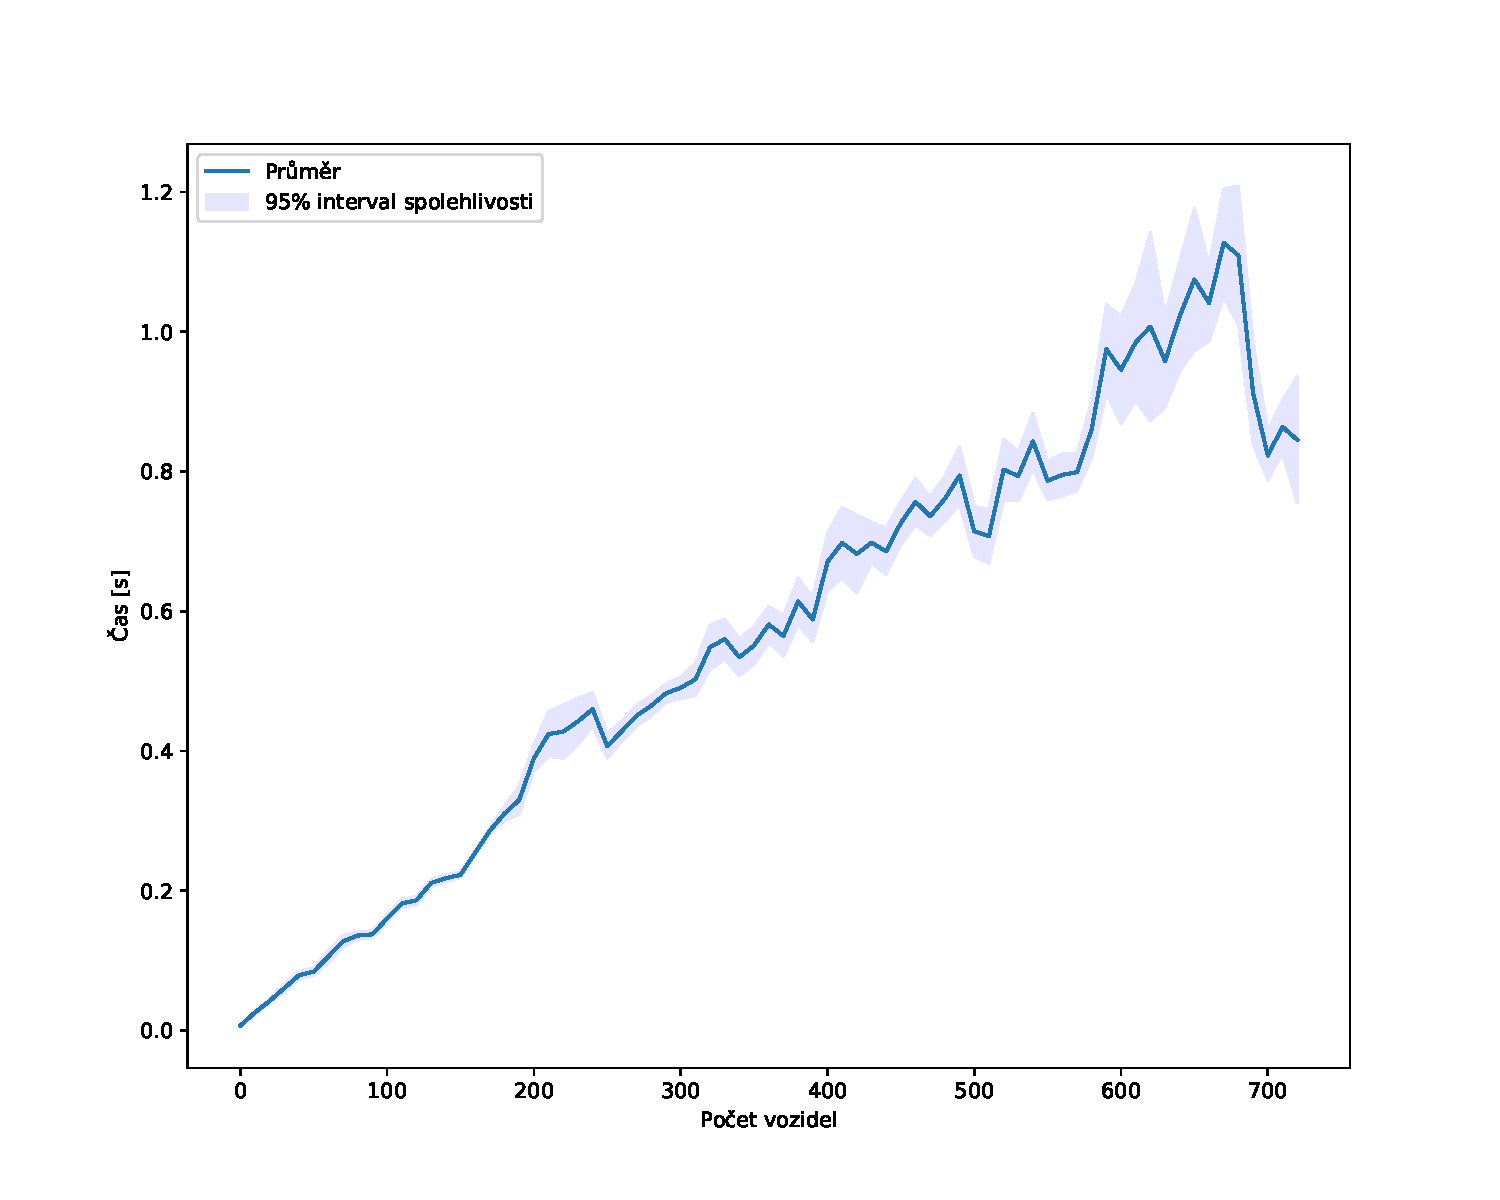
\includegraphics[width=0.7\linewidth]{../img/file_process_time}
  \caption{Průměrný čas zpracovávání daného počtu vozidel ze všech souborů se statickými daty. Světle modrá barva ohraničuje 95 \% interval spolehlivosti. Počty vozidel jsou vždy zaokrouhleny dolů na celé desítky.}
  \label{fig:file_process_time}
\end{figure}

\bigbreak

Jediné delší prodlení může nastat ve chvíli, kdy je potřeba stáhnout velké množství dodatečných informací o novém spoji. Na grafu \ref{fig:vehicle_pos_x_new_trips} je vidět, že až na jednotky vyjímek je počet nově nalezených spojů v jednom souboru nejvýše 20. Aplikace je ale naimplementována tak, aby se tyto informace stahovaly asynchroně a tedy čákání na stažení dat je co nejkratší.

\subsubsection{Konstrukce modelů}

Po využití testovacích dat vzorků poloh vozidel zaznamenaných ve dnech 20.--24. února 2020 bylo podle krytérií, kterými jsou zejména vzdálenost zastávek a počet vzorků mezi nimi, sestrojeno celkem 1106 polynomiálních modelů. Z toho je 847 modelů pro pracovní dny, které jsou nejdůležitější. Přičemž celkový počet párů zastávek je 7230, ale zastávek ve vzdálenosti 1500 metrů\footnote{zvolená minimální vzdálenost mezi zastávkama, mezi kterýma má ještě smysl odhadovat zpoždění} je pouze 2142. Z toho vychází, že u 40 \% dvojic zastávek je dostatek dat, aby dával výpočet modelu smysl.

\bigbreak

U zbylých dvojic zastávek se využívá lineární model.

\bigbreak

Čtení dat potřebných pro trénování modelů z databáze, kde jsou data ze 4 dnů trvá přibližně 110 sekund. Čtení se totiž provádí komlikovaným \gls{sql} datazem uvedeným v kapitole \ref{subsection:cteni_dat}, ovšem na rychlost provedení tohoto dotazu i konstrukce modelů celkem neklademe žádné časové nároky, protože přepočítávání modelů je plánováno na čas nejmenšího zatížení systému, což bývá typicky v noci, kdy máme několik hodin pro výpočet.

\bigbreak

Dále ověřme, že výsledek dotazu nezahltí paměť počítače, dotaz sice umožňuje čtení dat po stránkách, ale v implementaci se tato vlastnost nevyužívá. Určení velikosti objektu jazyka Python3 v paměti počítače není úplně trivální úloha, protože v paměti není objekt uložen na jednom místě, na jeho části se totiž ukazuje pointery\footnote{https://docs.python.org/3/reference/datamodel.html\#objects-values-and-types}. Dobrý odhad nám, ale poskytne objektu na disk pomocí knihovny \verb-pickle-\footnote{https://docs.python.org/3/library/pickle.html}. Takto uložený objekt zabírá necelých 10 MB prostoru na disku.

\bigbreak

Samotné zpracování dat a trénování modelů trvá pro všechny 2142 párů zastávek přes 2 minuty. Pro jeden pár zastávek je průměrná doba běhu 57 milisekund. Nejdéle trvá výpočet modelů 1.2 sekundy a to v případě, kdy se zpracovává dohromady přes 10 000 vzorků poloh vozidel.

\subsubsection{Serverová část uživatelské aplikace}

Server odpovídá na všechny typy požadovaných dotazů.

\bigbreak

Server je schopný odbavit přinejmenším 100 dotazů za sekundu. Na grafu \ref{fig:server_response_time} je zobrazeno jako dlouho trvalo serveru odpovědět na 100 paralelních dotazů, celkem ve 1 000 případech. Průměrně odpověd trvala mírně přes půlsekundu a jen v jednom případě jsme na odpověď čekali rovnou sekundu, což je nejzaší přípustná hodnota.

\begin{figure}
	\centering
  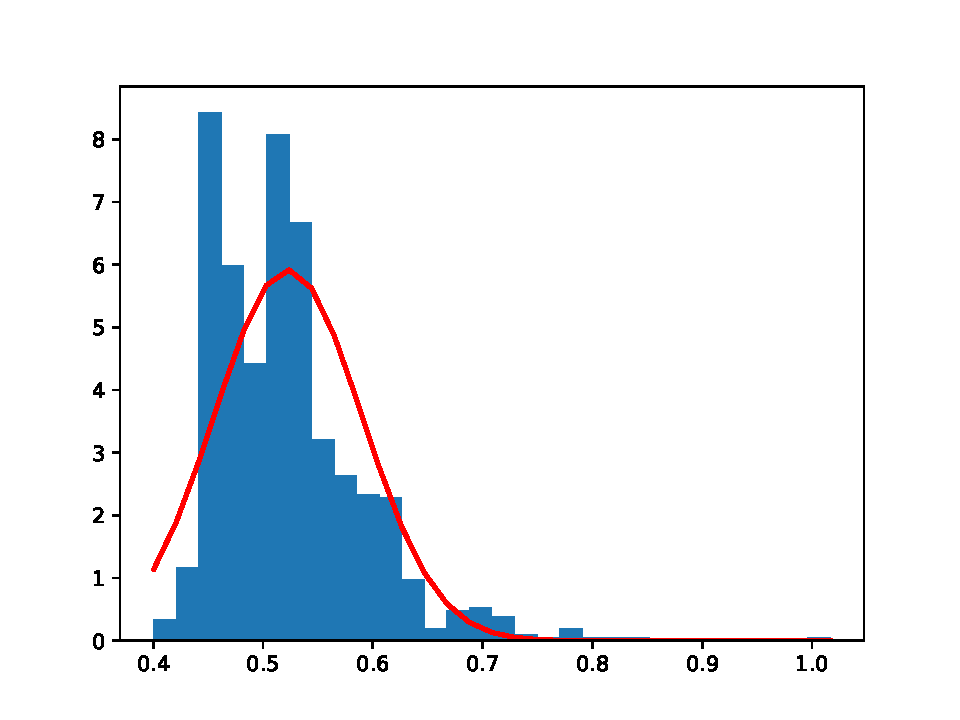
\includegraphics[width=0.7\linewidth]{../img/server_response_time}
  \caption{Doba odpovědi serveru na 100 paralelních dotazů (1000 vzorků)}
  \label{fig:server_response_time}
\end{figure}

\subsubsection{Vizualizace}

Zátěžové testování vizualizační aplikace se dělá poměrně obtížně. Prakticky je pro testování jakékoliv frondendové aplikace vždy potřeba spustit aplilaci na konkrétním zařízení a pozorovat její chování a výkon.

\bigbreak

V našem případě pro testování zobrazení voziddel na mapě se spokojíme s testováním ve webovém prohlížeči, konkrétně v Safari verze 14.0.3 a Google Chrome verze 90.0.4430.93. Testování probíhá na datech používaných pro demonstraci běhu celého řešení. Tato data jsou sesbírána ve dne 23. 2. 2020 večer a zachycují půlhodinový časový interval.

\bigbreak

Oba prohlížeče bez jakýchkoli problémů zobrazily v jeden moment více než 100 vozidel a stejně tak zvládly i data aktualizovat. Po celou dobu testování aplikace běžela plynule. Ukázky grafického znázornění jsou zobrazeny na obrázcích \ref{fig:dve_vozidla}, kde je vybrán jeden spoj a zobrazují se jeho zastávky a jeho trasa. Dále na obrázku \ref{fig:big_picture} jsou vidět polohy vozidel tak, jak byly zaznamenány 23. 2. 2020 ve 21:30. Na obrázku \ref{fig:cluster} je zobrazen způsob zobrazení shluku vozidel, ikony reprezentující vozidla se překrývají, zároveň ale překryvy nepůsobí nijak rušivým dojmem, navíc po přejetí myší po jakékoli části i částečně skryté ikony přenese ikona do popředí tak, aby bylo číslo linky dobře viditelné a bylo umožněno vybrání vozidla klikem myši.

\begin{figure}
	\centering
  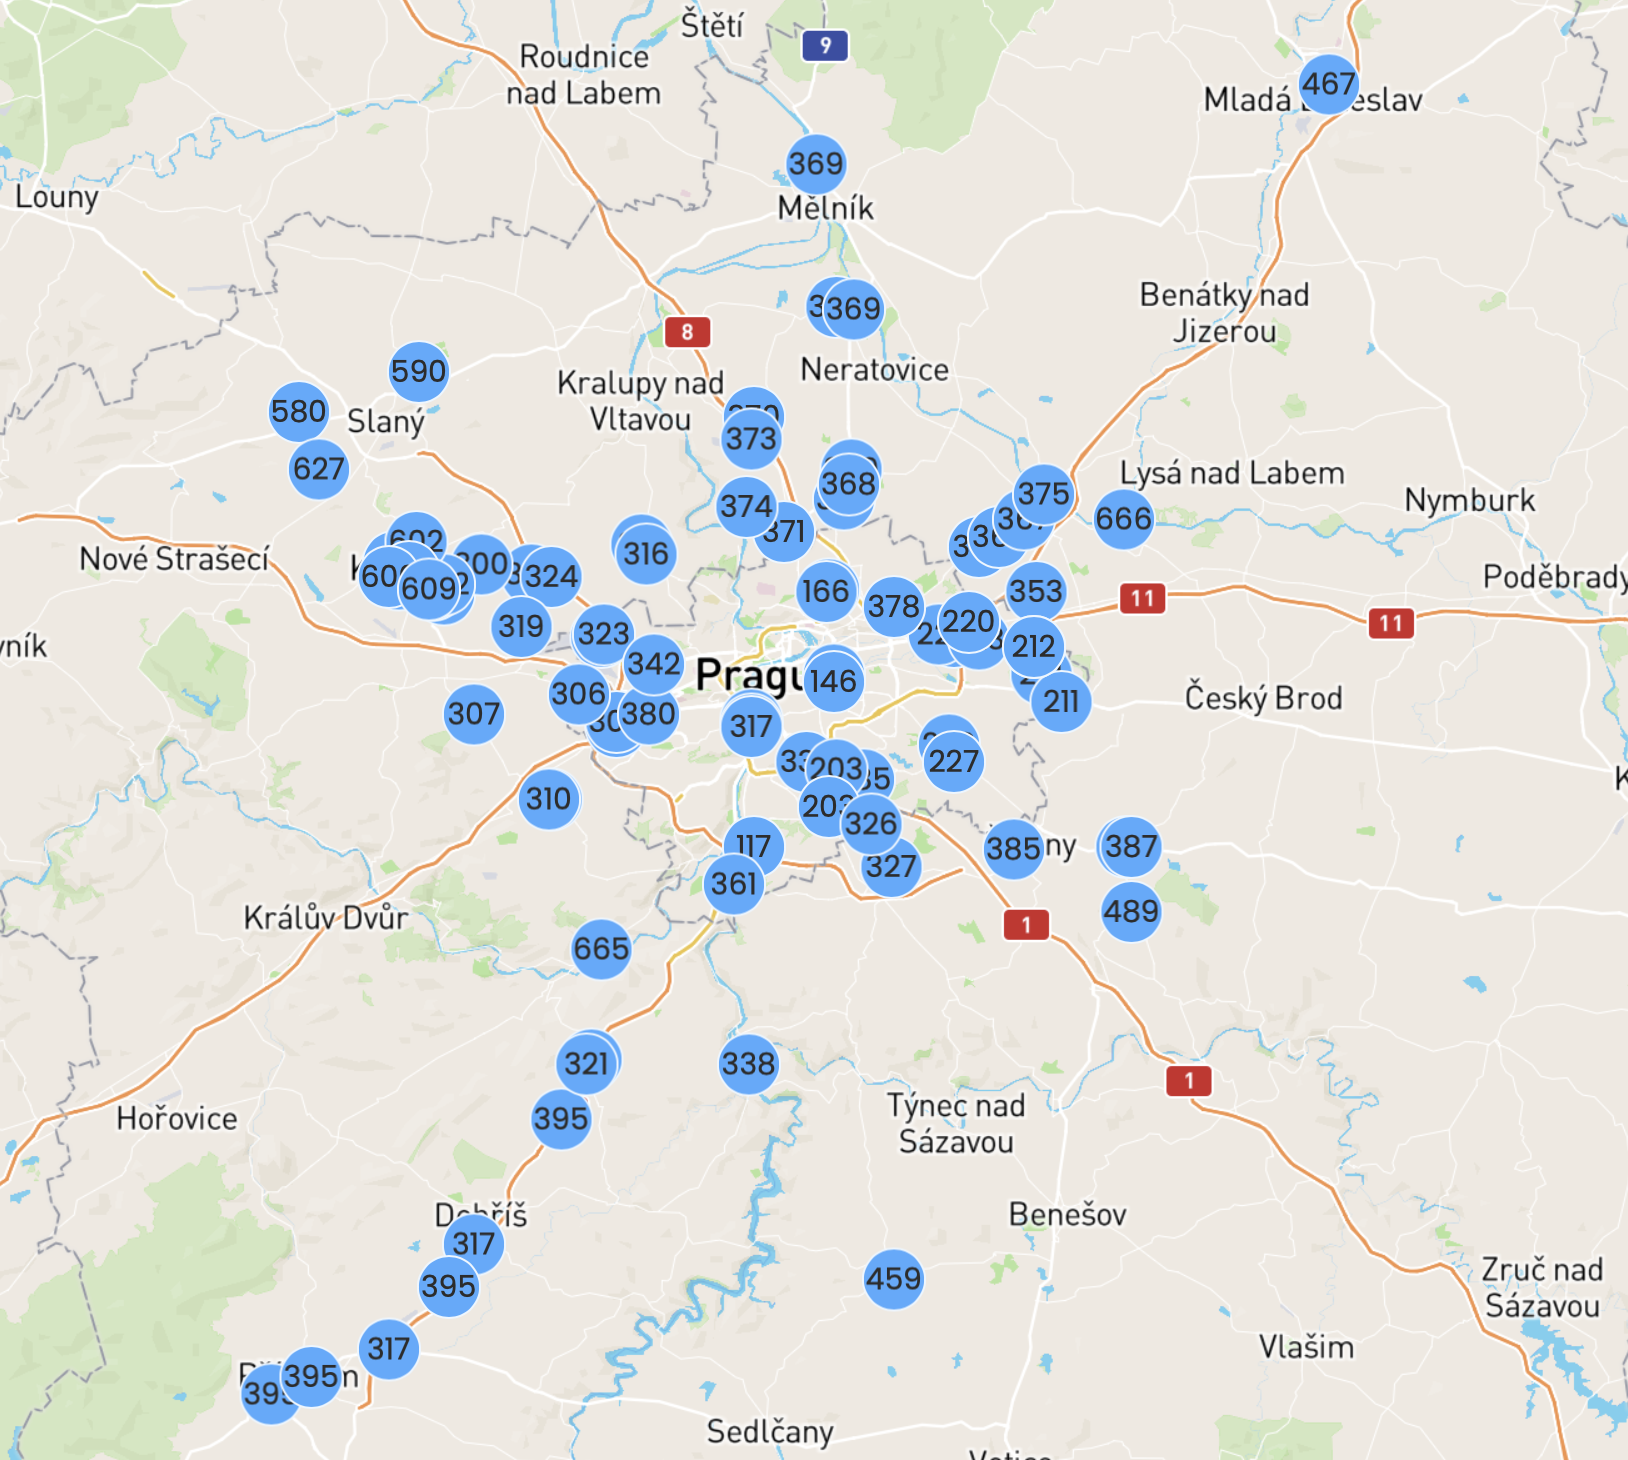
\includegraphics[width=0.7\linewidth]{../img/big_picture.png}
  \caption{Mapa Prahy a okolí s polohy vozidel zaznamanány 23. 2. 2020}
  \label{fig:big_picture}
\end{figure}

\begin{figure}
	\centering
  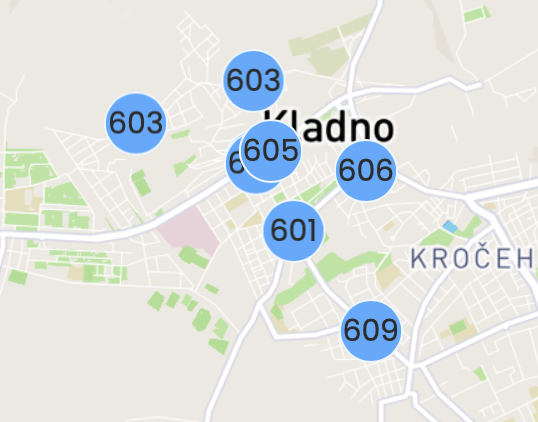
\includegraphics[width=0.3\linewidth]{../img/cluster.png}
  \caption{Shluk vozidel}
  \label{fig:cluster}
\end{figure}


\bigbreak

Dále se v pořádku zobrazily i přídavné informace o vybraném vozidle. Tedy všechny zastávky, kterými spoj projíždí, kterých může být i několik desítek a tabulka s jízdním řádem. Na obrázku \ref{fig:trip_path} je vidět zobrazení celé trasy spoje. Vybraný spoj je zvýrazněn a vždy se zobrazí přes všechny ostatní ikony jiných vozidel. Jízdní řád spoje se pak zobrazí v tabulce zobrazené na obrázku \ref{fig:kladno_aut_322}.

\begin{figure}
	\centering
  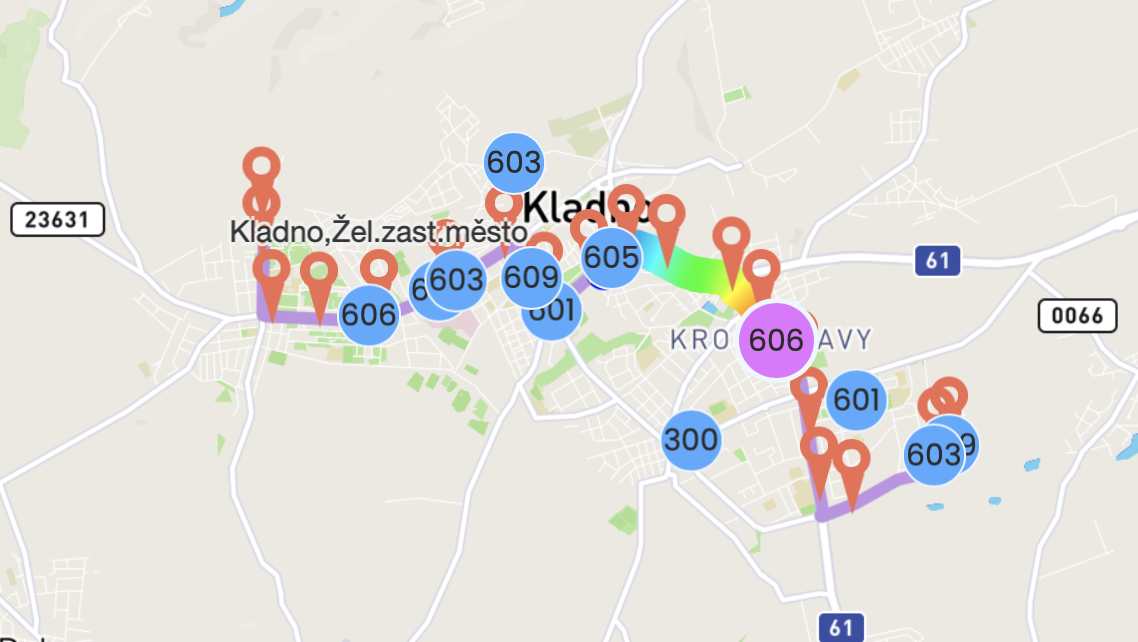
\includegraphics[width=0.7\linewidth]{../img/trip_path.png}
  \caption{Vyznačená trasa jízdy}
  \label{fig:trip_path}
\end{figure}

\begin{figure}
	\centering
  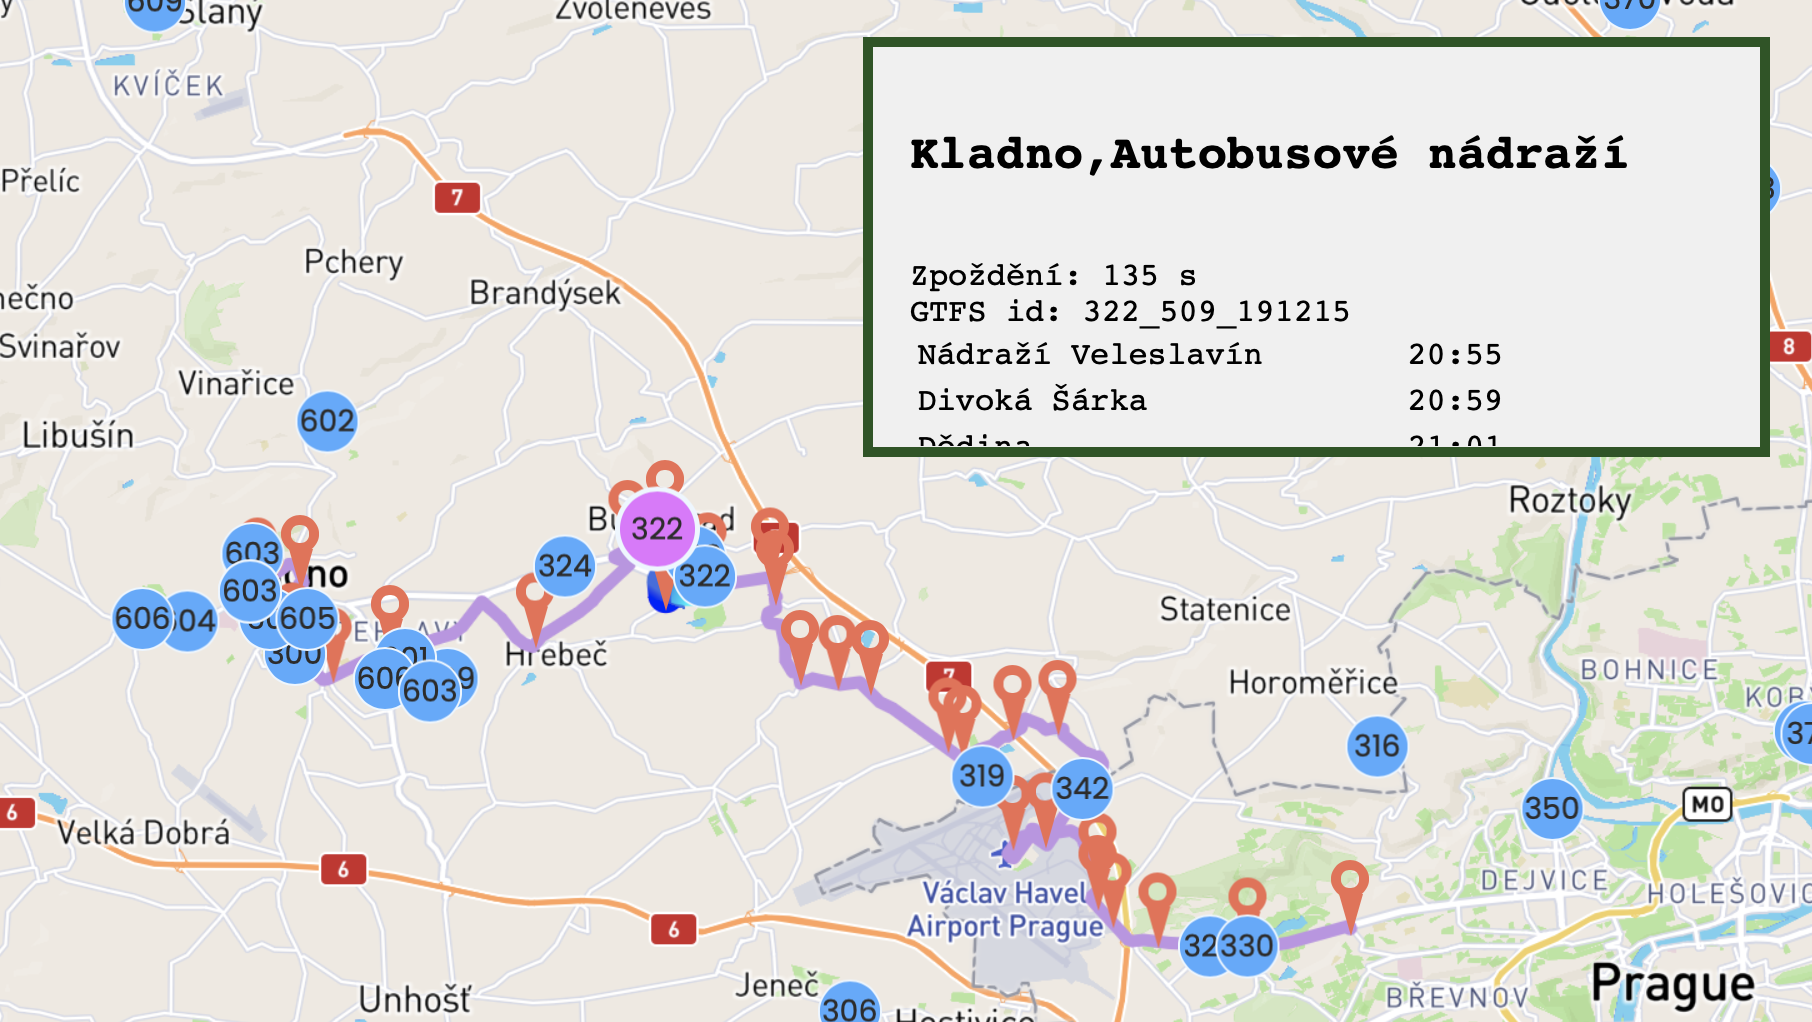
\includegraphics[width=0.7\linewidth]{../img/kladno_aut_322.png}
  \caption{Vyznačená trasa jízdy s jízdním řádem}
  \label{fig:kladno_aut_322}
\end{figure}

\bigbreak

Pokud byla vybrána zastávka zobrazila se odjezdová tabule a všechny spoje, které budou zastávkou projíždět\footnote{V demonstrační aplikaci se zobrazí všechny spoje projíždějící zastávkou, protože časy jízdních řádů neodpovídají simulovaným časům pořízení vzorků poloh vozidel.}. Zobrazení více vozidel současně je ilustrováno na obrázku \ref{fig:more_trips}. Odjezdová tabule je zobrazena na obrázku \ref{fig:stredokluky_table}

\begin{figure}
	\centering
  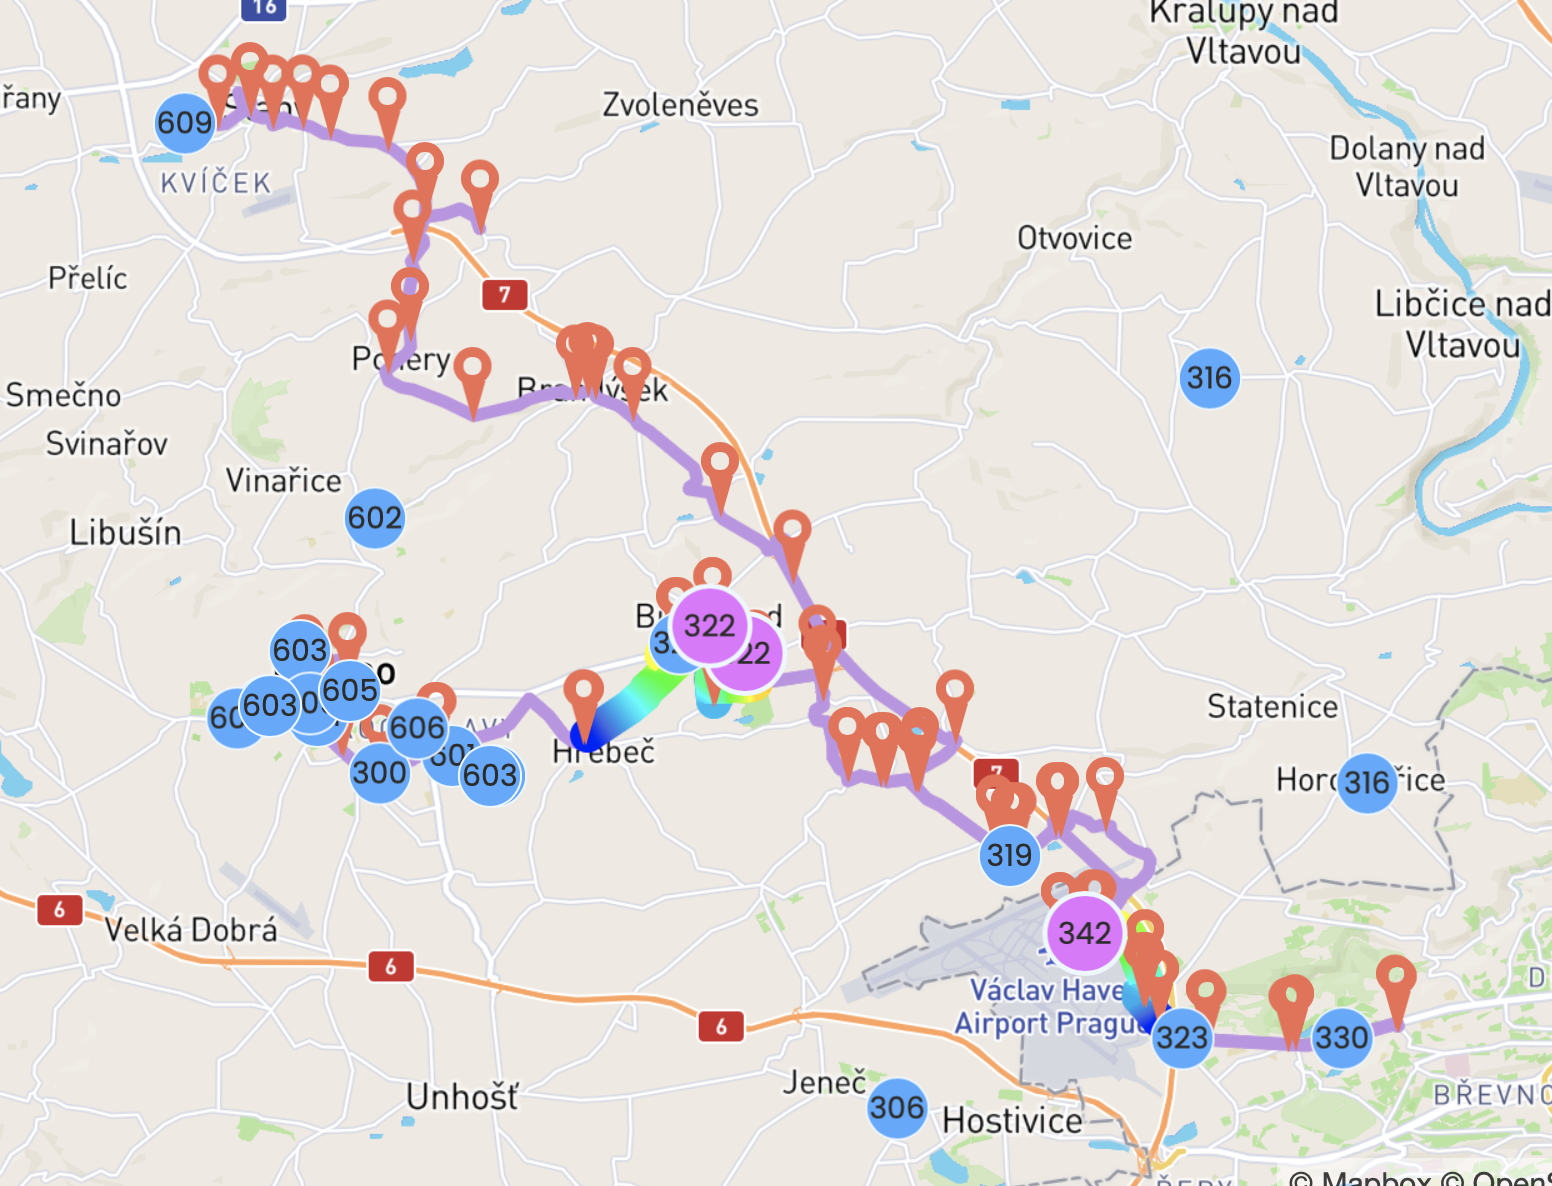
\includegraphics[width=0.7\linewidth]{../img/more_trips.png}
  \caption{Vozidla projíždějící vybranou zastávkou}
  \label{fig:more_trips}
\end{figure}

\begin{figure}
	\centering
  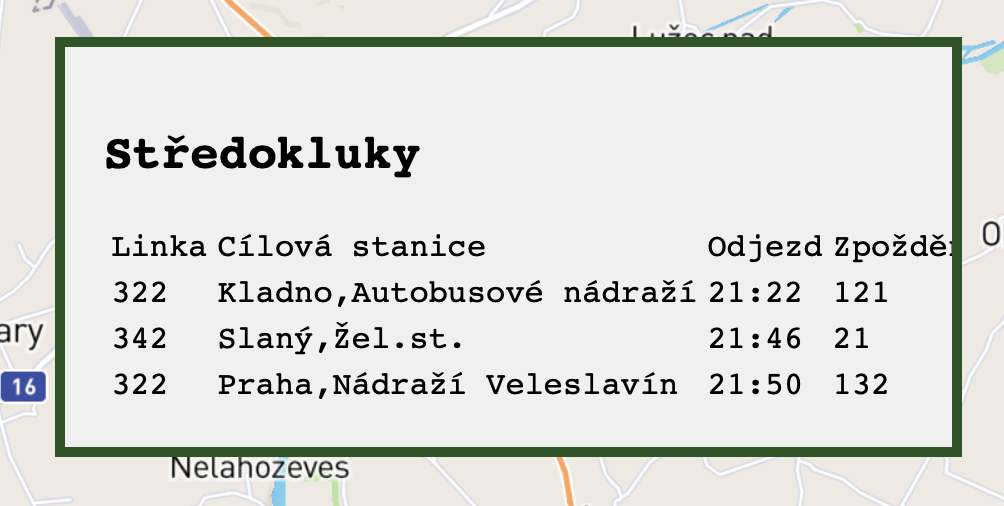
\includegraphics[width=0.4\linewidth]{../img/stredokluky_table.png}
  \caption{Odjezdová tabule}
  \label{fig:stredokluky_table}
\end{figure}

\section{Evaluace výsledků}

\subsection{Konstrukce modelů}

Zde popsaná data vychází z trénování modelů na datech sbíraných ve dnech 20. 2. 2020 -- 23. 2. 2020, tedy ze 4 dnů (2 pracovních, 2 víkendových).

\bigbreak

Z 2142 dvojic zastávek se alespoň pro jeden typ dne (pracovní, víkendový) vytvořil polynomiální model popisující profil jízdy mezi nimi pro 1108 dvojic zastávek. Pro oba typy dnů se polynomiální model vytvořil ve 222 případech. Ve 190 případech se vytvořil model pouze pro pracovní dny protože mezi danou dvojcí zastávek nejel žádný spoj ve víkendový den.

\bigbreak

Chceme-li zjisti jak přesně jsou profily jízdy odhadnuty pomocí vytvořených modelů, zaměříme se na \gls{rmse} u každého modelu. Tato chyba nám říká o kolik sekund se v průměrném případě náš odhad plete od skutčnosti na testovacích datech\footnote{Jedná se o testovací data, podle kterých se určil nejlepší stupeň polynomu. Kdy vstupní data pro funkci trénování modelu byla rozdělena na trénovací a testovací. Testovací data podle kterých posuzujeme vlastnosti nově odhadnutých zpoždění v kapitole \ref{subsection:odhady_zpozdeni} je zcela jiná množina dat.}. Pro pracovní dny je průměrná \gls{rmse} necelých 20 sekund. Nejvyšší \gls{rmse} byla zaznaménana 200 sekund. Tak vysoké odchylky jsou, ale po prozkoumání jednotlivých případů způsobeny chybami ve vstupních datech, které se automaticky odstraňují jen velmi obtížně, příklad je zobrazen na grafu \ref{fig:chyba_zpozdeni_v_posledni_zastavce}. V tomto konkrétním případě jsou chybně uvedena zpoždění v poslední projeté zastávce. Histogram všech \gls{rmse} modelů z pracovních dnů je zobrazen na grafu \ref{fig:rmse}. Zde je patrné, že nejčastěji je chyba do 30 sekund a zcela výjmečně překročí 60 sekund. Takto nízké chyby jsou nad očekávání dobré, protože průměrných 20 sekund je pro cestujícího čekající na autobus takřka nepostřehnutelných.

\begin{figure}
	\centering
  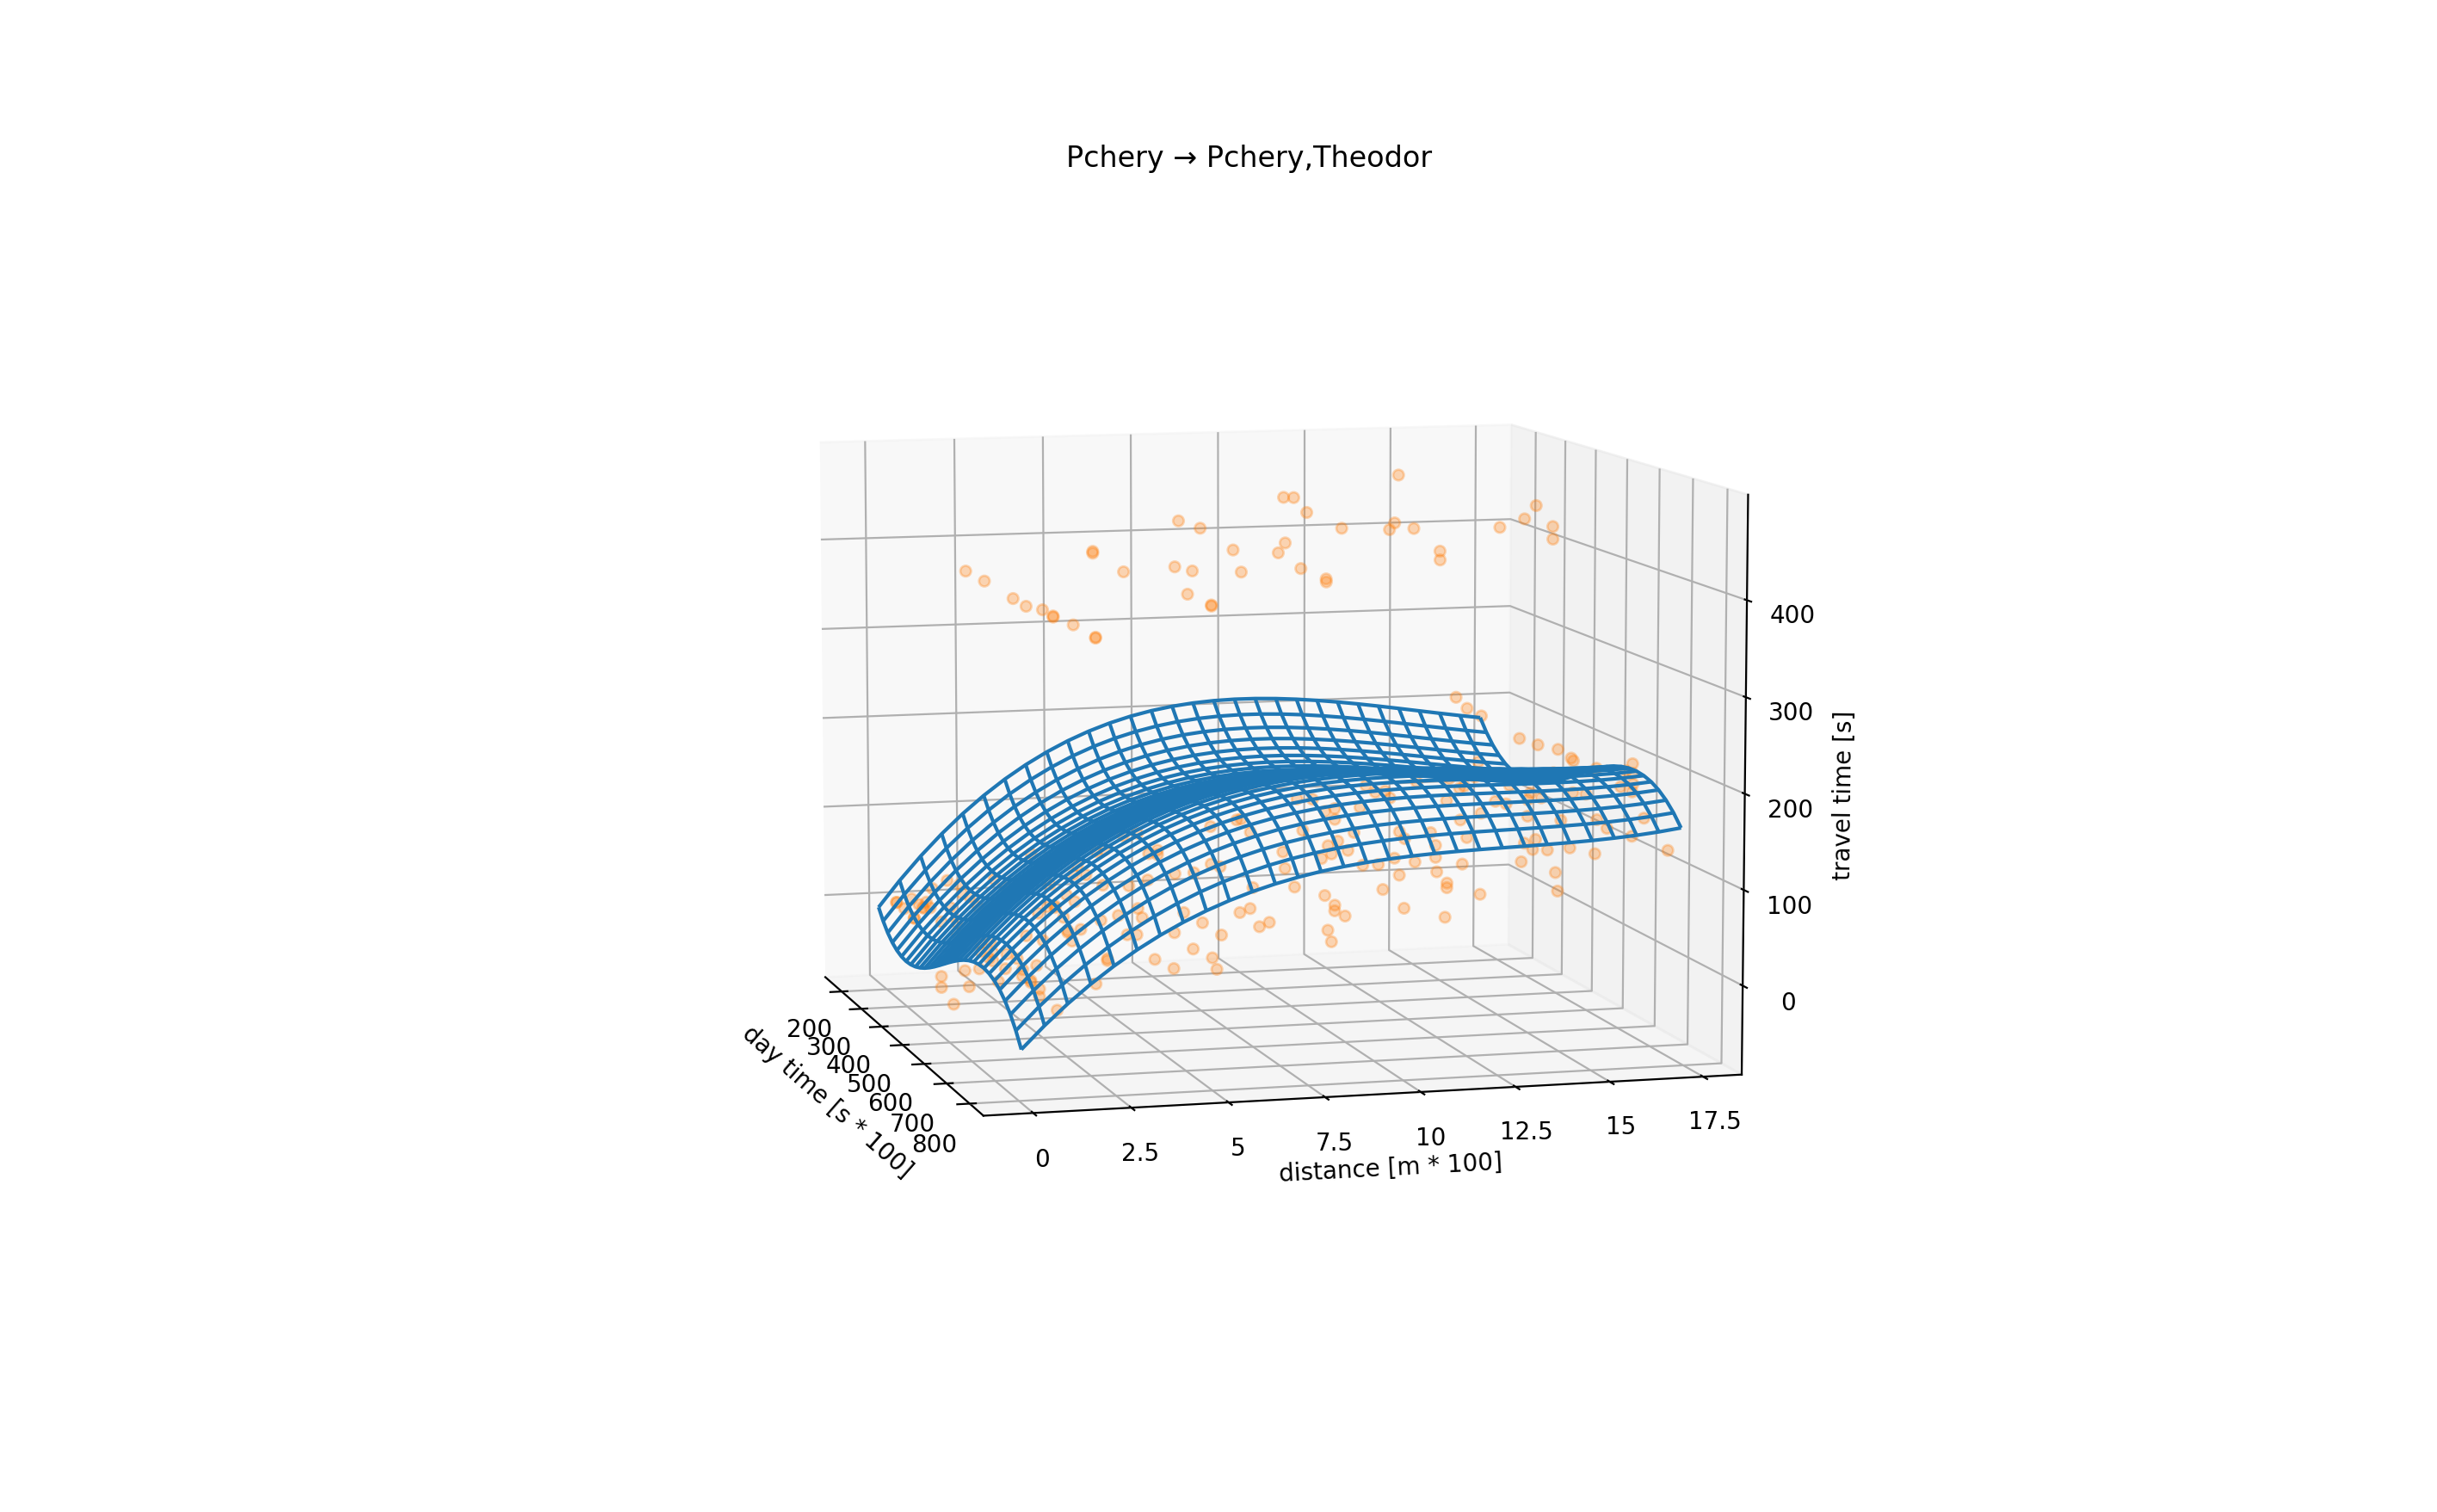
\includegraphics[width=0.4\linewidth]{../img/chyba_zpozdeni_v_posledni_zastavce.png}
  \caption{Modelování profulu jízdy s chybnými vstupními daty}
  \label{fig:chyba_zpozdeni_v_posledni_zastavce}
\end{figure}

\begin{figure}
	\centering
  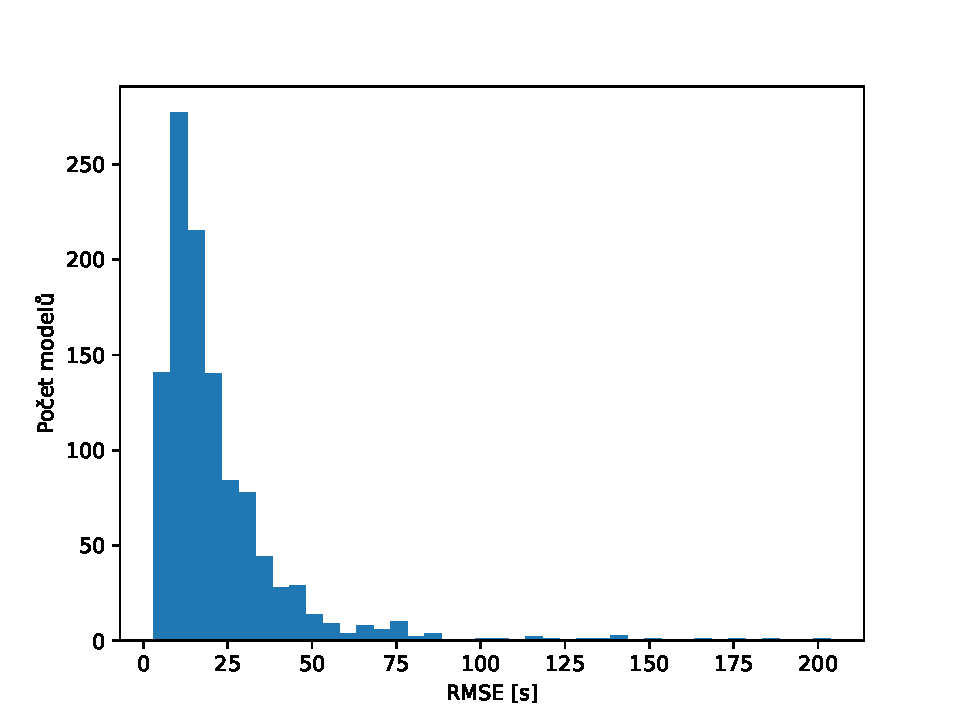
\includegraphics[width=0.4\linewidth]{../img/rmse}
  \caption{Histogram \gls{rmse}}
  \label{fig:rmse}
\end{figure}

\bigbreak

Co se týče stupňů polynomiálních regresí, které využíváme při konstrukci modelů, tak nejčastěji se generoval model stupně 3 nebo 4. Což značí, že průběhy tras jsou poměrně tvárné. Modely vyššího stupně se nalezly také, ale spíše značí chybu v datech, protože se tak snaží vymodelovat různě rozházené vzorky jako třeba na obrázku \ref{fig:chyba_zpozdeni_v_posledni_zastavce}. Nakonec se nalezlo i nezanedbatelné množství modelů stupně 2, což také značí tvárnost, ale převážně jen v jedné ose. Vizualizace modelu druhého řádu je na grafu \ref{fig:second_degree}, třetího řádu na grafu \ref{fig:thrd_degree}


\begin{figure}
	\centering
  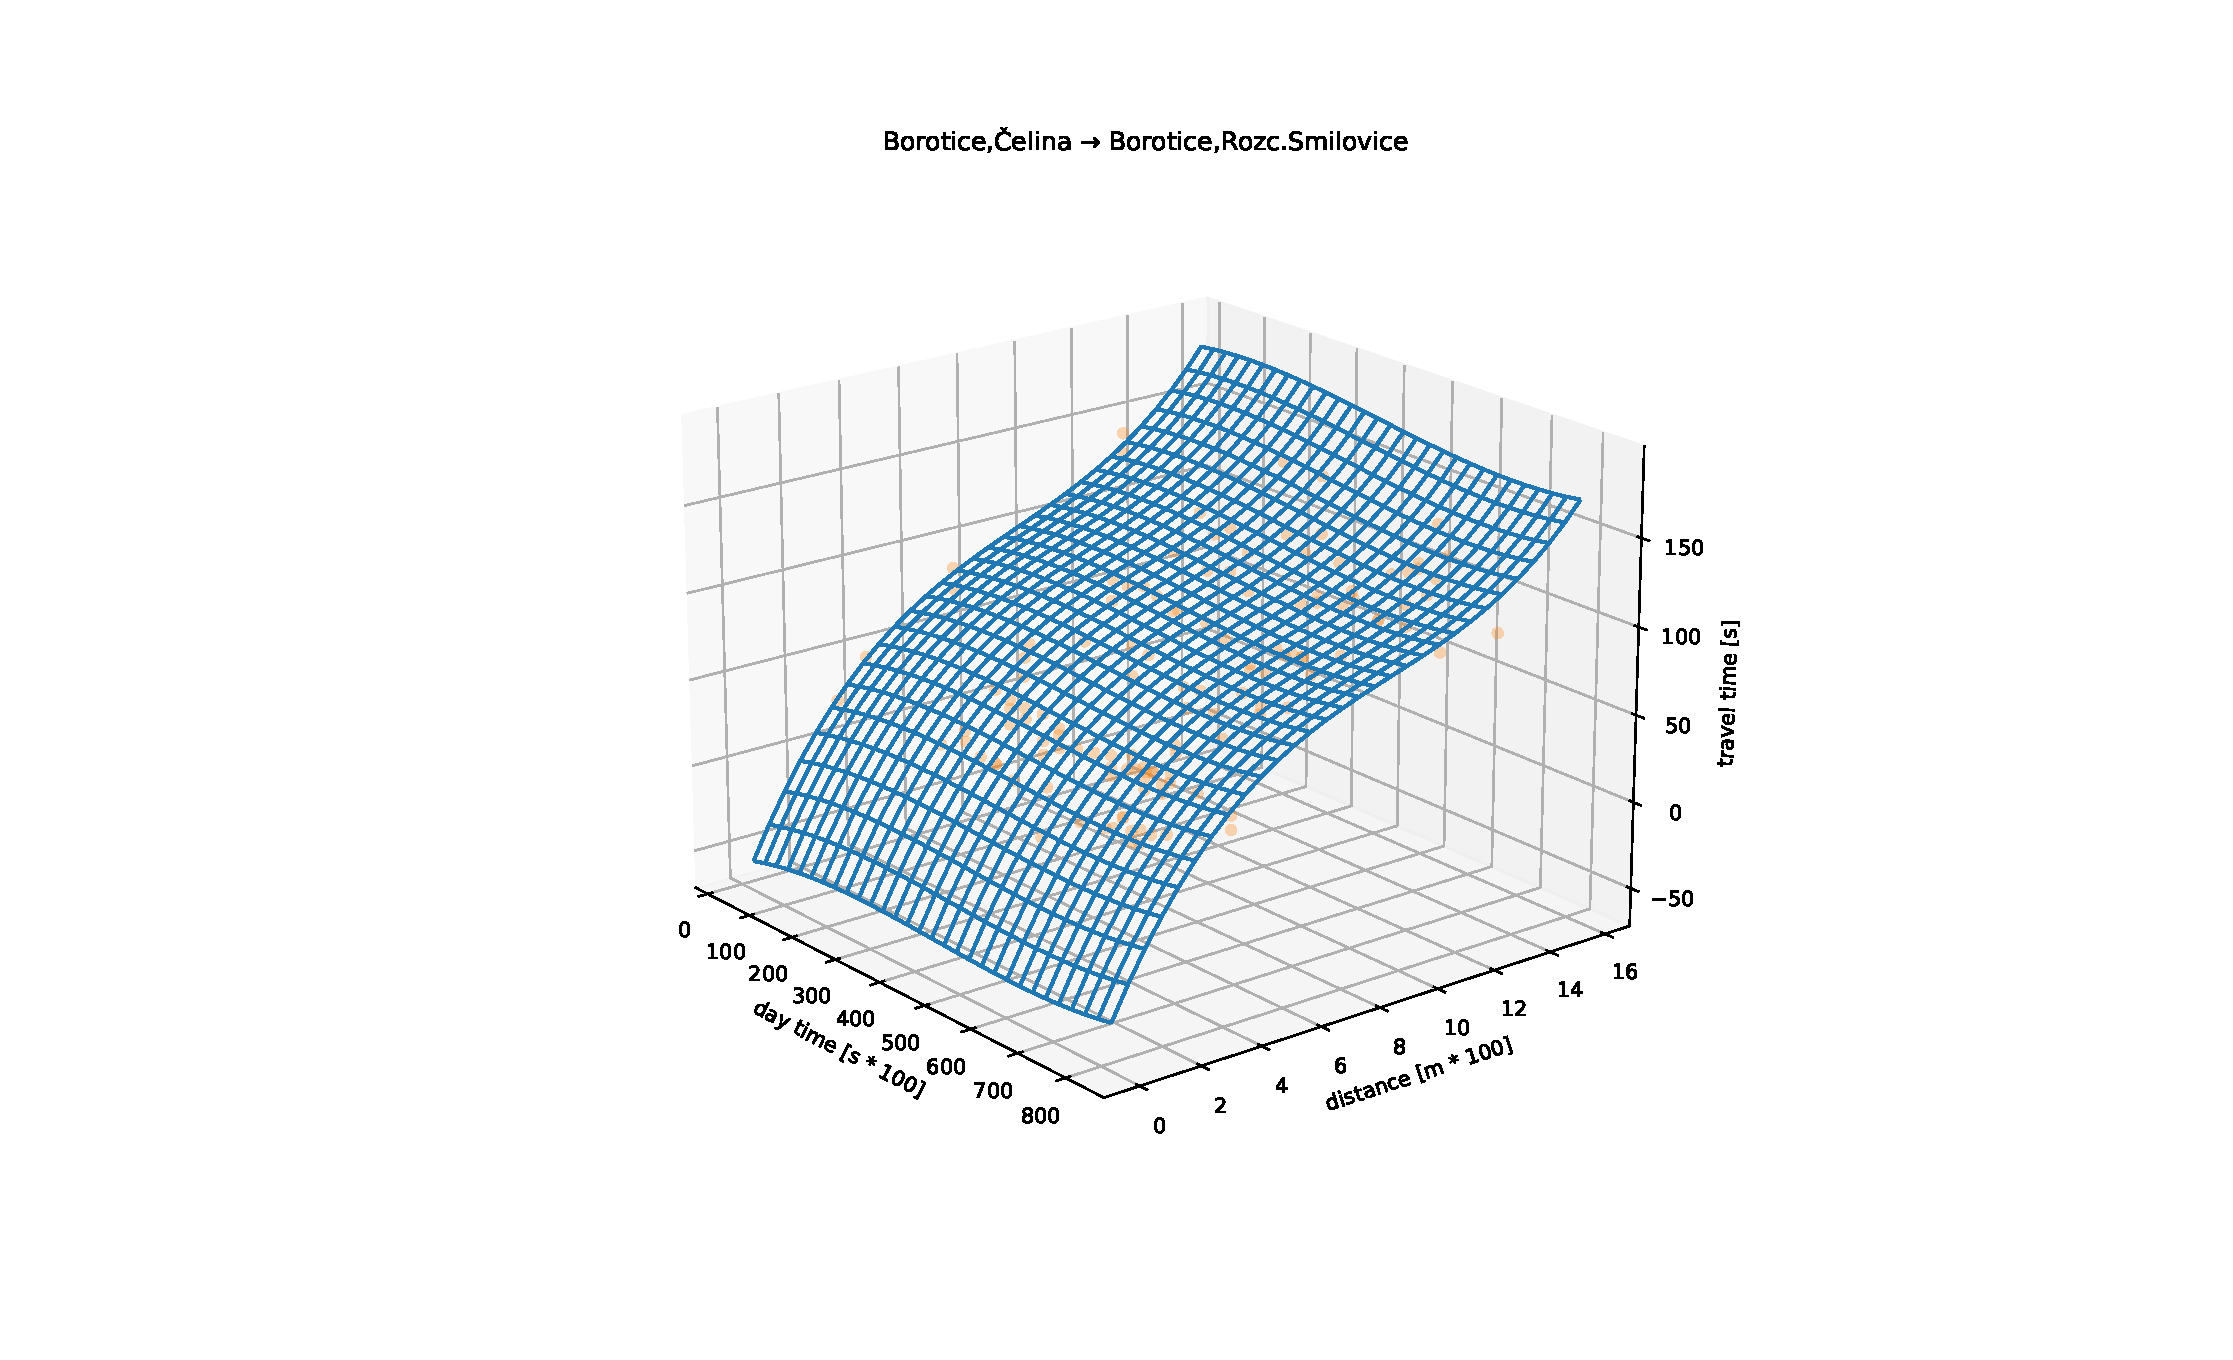
\includegraphics[width=1\linewidth]{../img/second_degree}
  \caption{Histogram \gls{rmse}}
  \label{fig:second_degree}
\end{figure}


\begin{figure}
	\centering
  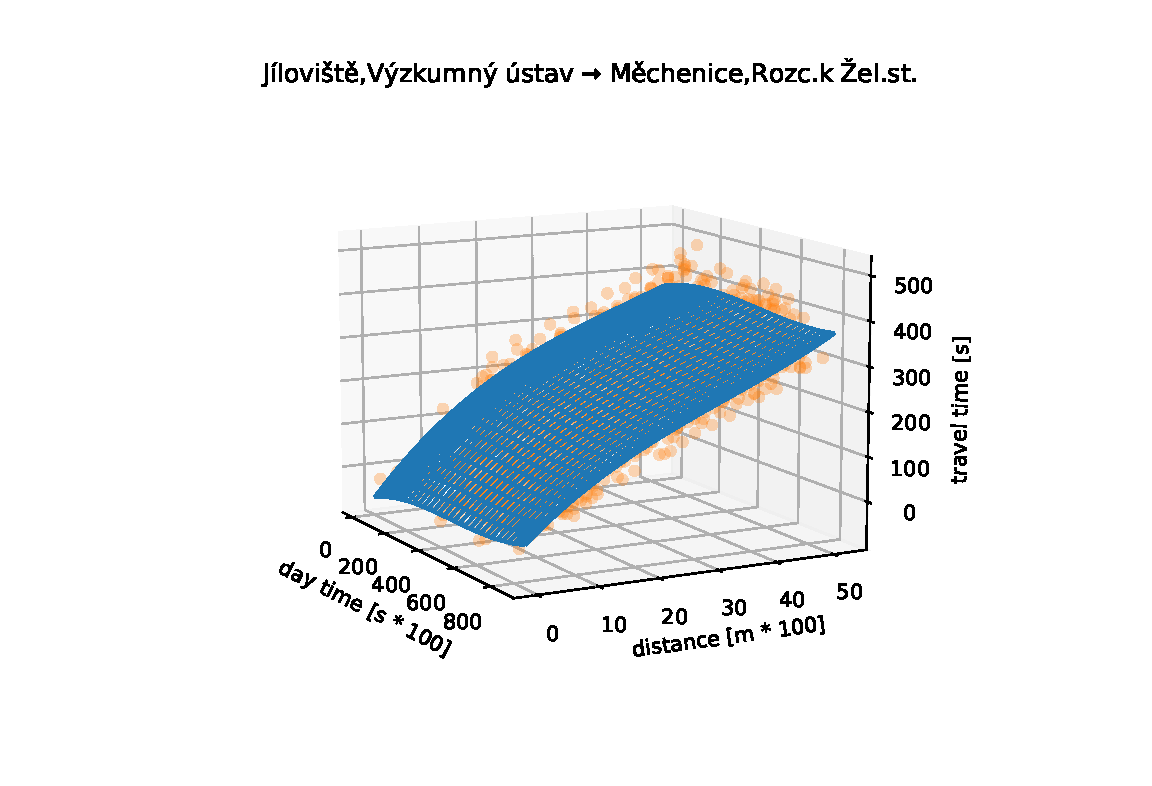
\includegraphics[width=1\linewidth]{../img/thrd_degree}
  \caption{Histogram \gls{rmse}}
  \label{fig:thrd_degree}
\end{figure}


\subsection{Odhady zpoždění} \label{subsection:odhady_zpozdeni}

Z toho jak jsou definovány požadavky řešení v kapitole \ref{subsubsection:kvalitativni_pozadavky} pro změření kvality výsledků stačí porovnávat odhad zpoždění lineárního (původního) modelu a nového polynomiálního modelu. Přičemž odhad je lepší pokud má sekvence odhadů zpoždění z celé jízdy mezi dvojcí zastávek menší rozptyl.

\bigbreak

Podívejme se tedy na porovnání odhadů zpoždění novými modely profilů jízd se stávajícím řešení pracujícím s předpokladem, že vozidla jedou celou trasu mezi dvěma zastávkami konstantní rychlostí.

\bigbreak

Evaluaci výsledků budeme provádět s daty sesbíranými 20. 2. 2020, které použijeme jako trénovací data a s daty sesbíranými 21. 2. 2020, které použijeme jako testovací data. Toto je standardní postup pro hodnocení úspěšnosti predikcí modelů ve světě strojového učení. Modely nemohou být testovány na stejných datech, jako na kterých byly trénovány, protože kdyby se trénovalo i testovalo na stejných datech, model by nemusel nic predikovat, ale stačilo by, aby si jen "zapamatoval" hodnotu z množiny trénovacích dat.

\bigbreak

TODO

\section{Statistiky}

TODO
